\documentclass[12pt]{article}

% Use Times-like font for pdfLaTeX
\usepackage{mathptmx}

% Set up page geometry
\usepackage[a4paper, margin=1in]{geometry}
\usepackage[utf8]{inputenc}
\usepackage[T1]{fontenc}
\usepackage[ngerman]{babel} % Use 'english' for English text
\usepackage{amsmath}
\usepackage{graphicx}
\usepackage{geometry}
\usepackage{booktabs} % For professional tables
\usepackage{hyperref}
\usepackage{parskip} % Space between paragraphs

% Header and footer
\usepackage{fancyhdr}
\pagestyle{fancy}
\fancyhead[L]{Grundlagen der Raumfahrt}
\fancyhead[C]{Raketen-Flugsimulator}
\fancyhead[R]{Lorenz Saalmann}
\fancyfoot[C]{\thepage}

\begin{document}

\setlength{\parindent}{0pt}

% Document starts here

\begin{titlepage}
    \centering
    \begin{figure}
        \centering
        
\includegraphics[width=0.3\textwidth]{images/jlu_logo.jpeg}
    \end{figure}
    \vspace*{2cm}
    \Large{Praktikumsaufgabe Raketen-Flugsimulator} \\
    \vspace{2cm}
    \normalsize{Lorenz Saalmann (8104072)} \\
    \vfill
    \normalsize{{Grundlagen der Raumfahrt, WS 24/25}} \\
    \small{Sebastian Karl, Martin Grabe} \\
    \begin{figure}[h]
        \centering
        
\includegraphics[width=0.15\textwidth]{images/DLR_logo.png}
    \end{figure}
\end{titlepage}

\newpage

\section{Raketen-Flugsimulator}
Zunächst soll ein Programm zur Lösung der vereinfachten Bewegungsgleichungen für den Aufstieg einer zweistufigen Rakete geschrieben werden. Dafür wurden die Bewegungsgleichungen (1.20) aus Abbildung \ref{fig:equations} verwendet. Für eine Abschätzung des Luftwiderstands wurde folgender exponentieller Zusammenhang verwendet:
\begin{equation}
    \rho(h) = 1.2 \, \frac{\text{kg}}{\text{m}^3} \exp \left( -1.244268 \cdot 10^{-4} \, \text{m}^{-1} \cdot h \right)
\end{equation}

\begin{figure}
    \centering
    \label{fig:equations}
    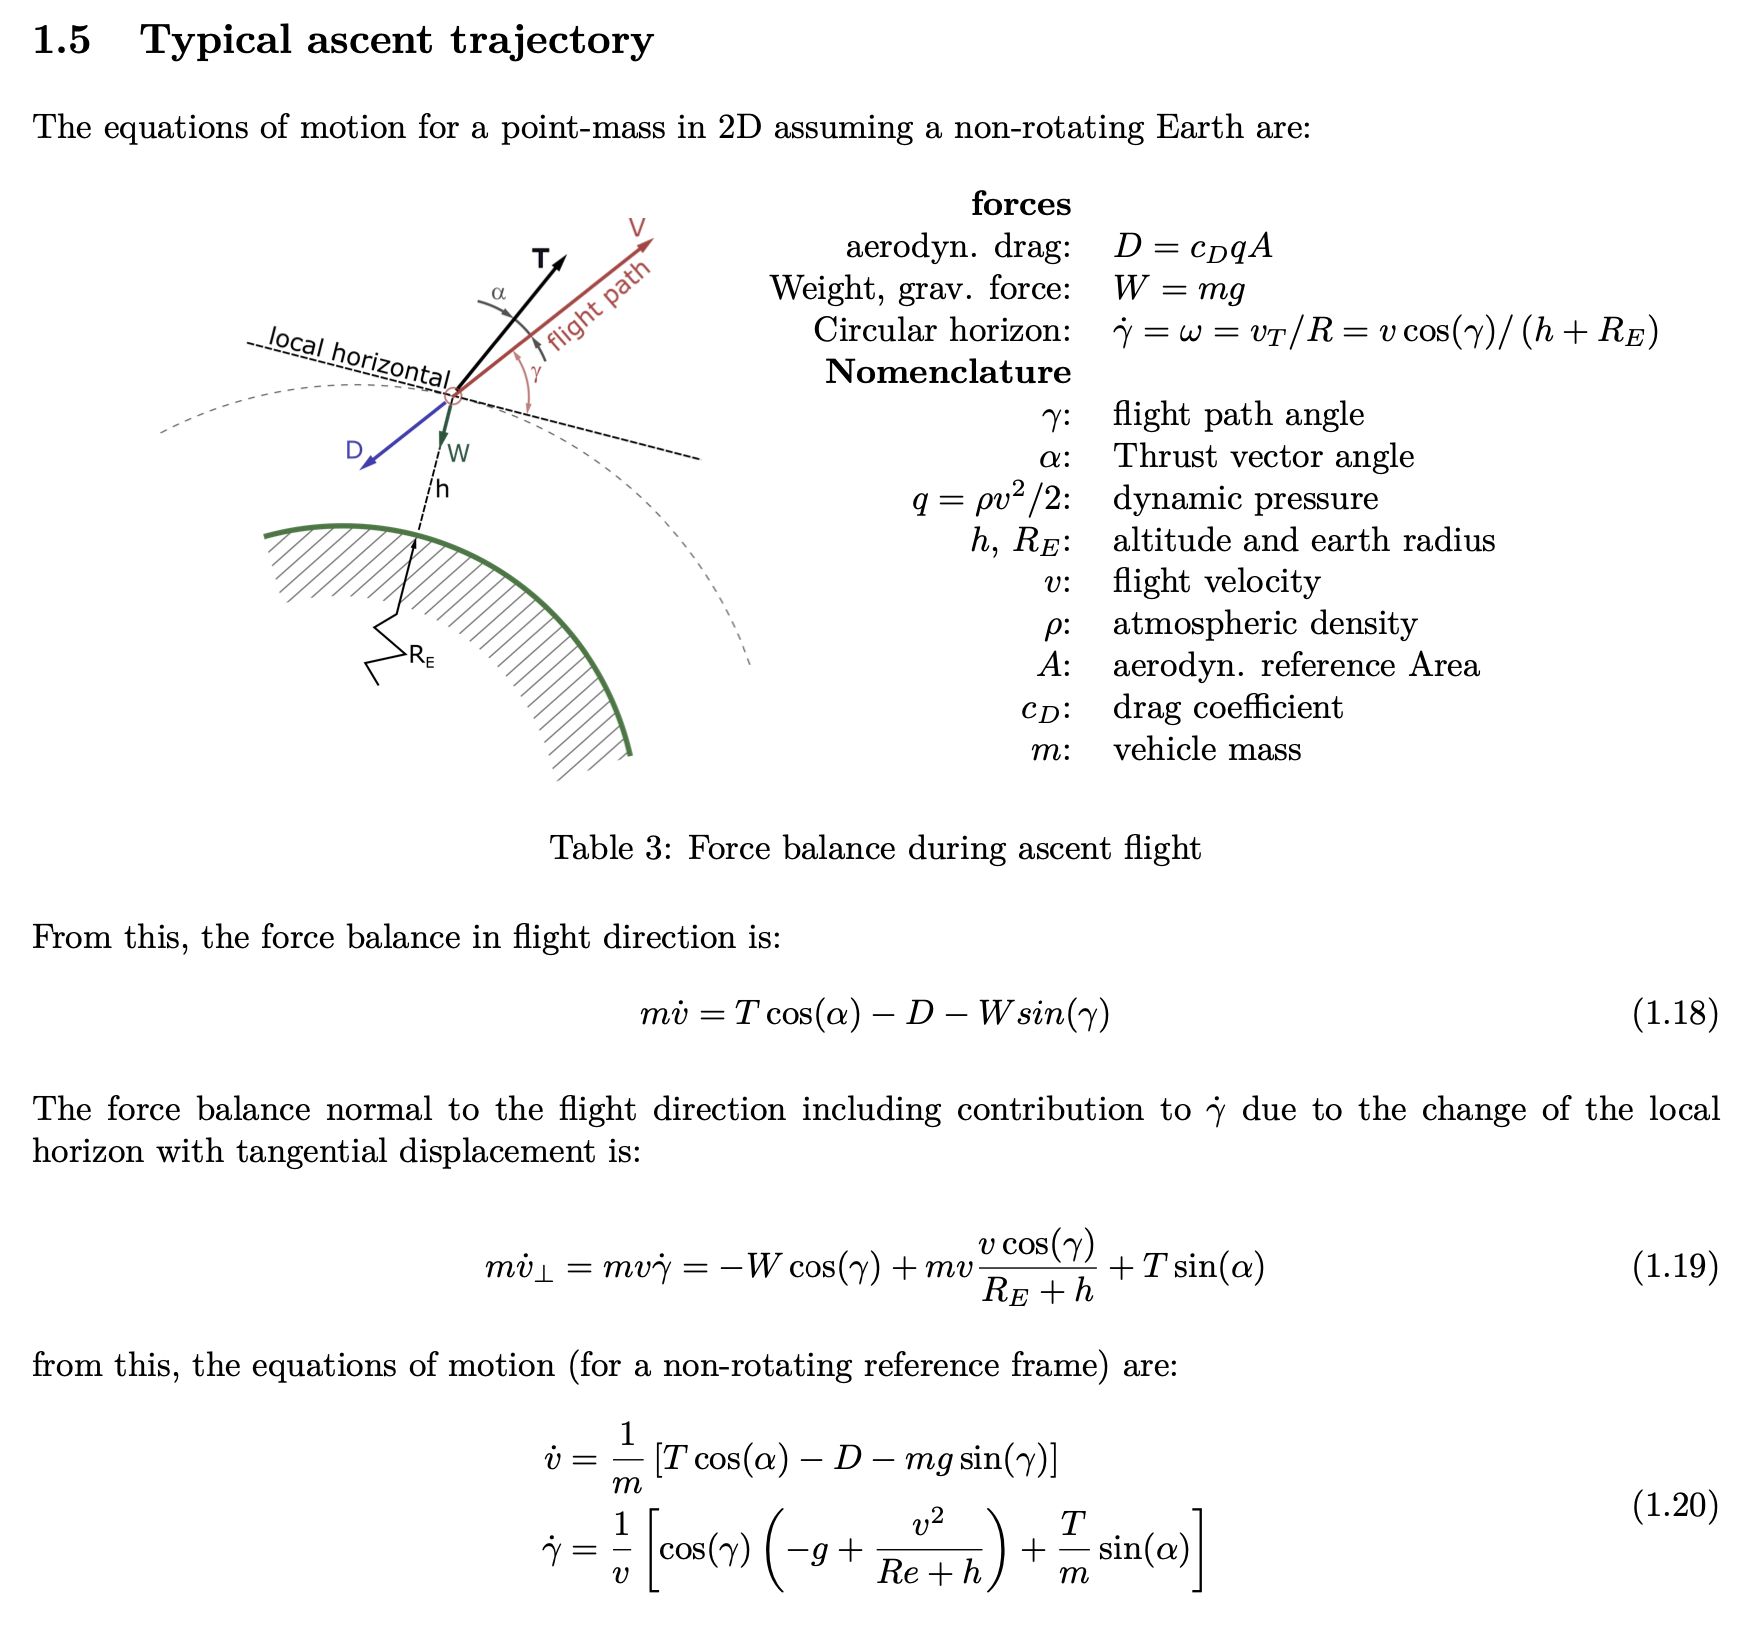
\includegraphics[width=1\textwidth]{images/equations.png}
    \caption{Herleitung der Bewegungsgleichungen für den Raketenflug aus dem Vorlesungsskript}
\end{figure}

Die effektive Querschnittsfläche soll $A = 15 \, \text{m}^2$ betragen, der Widerstandsbeiwert ist $C_D = 1$. Weiterhin soll die Abnahme der Erdanziehungskraft mit der Flughöhe berücksichtigt werden. Der Zielorbit kann mit einem TVC erreicht werden, bei dem der Schubvektor zwischen einer Flughöhe von 250 und 3000 m um 3$^\circ$ ausgelenkt wird.

Das Programm wurde in Python umgesetzt. Es besteht im Wesentlichen aus drei Skripten: \textit{main.py} ist der Startpunkt des Programms, \textit{flight-sim.py} simuliert die Differentialgleichungen iterativ und \textit{plotter.py} stellt die Ergebnisse graphisch dar. Die Ausgabe des Programms ist in Abbildung \ref{fig:output} zu sehen. Hier sind auch die Geschwindigkeit, die Flughöhe und die Masse über die Zeit dargestellt. Zusätzlich wurde der Flugbahnwinkel der Rakete über der Zeit in Abbildung \ref{fig:angle} dargestellt. 
\begin{figure}
    \centering
    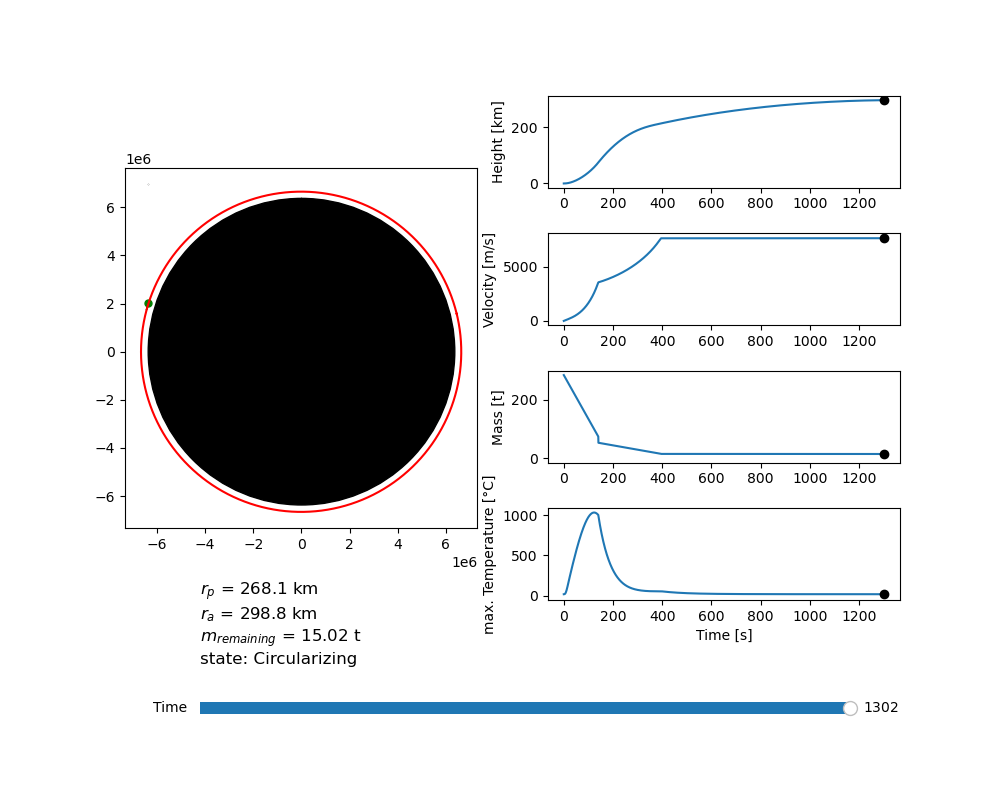
\includegraphics[width=1\textwidth]{images/output.png}
    \caption{Beispielhafte Ausgabe des Raketen-Flugsimulators am Besipiel für Aufgabe 1}
    \label{fig:output}
\end{figure}

\begin{figure}
    \centering
    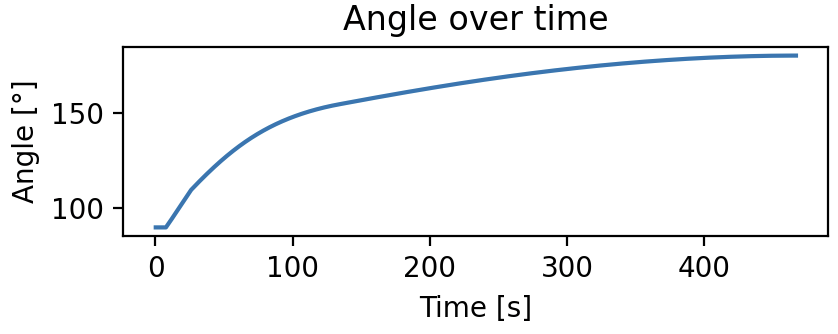
\includegraphics[width=.8\textwidth]{images/angle_over_time.png}
    \caption{Flugbahnwinkel der Rakete über der Zeit}
    \label{fig:angle}
\end{figure}

\subsection{Weitere Aufgaben}
\begin{enumerate}
    \setcounter{enumi}{2}
    \item  \textbf{Wie viel Treibstoff ist beim Erreichen des Orbits noch übrig?} \\
    Beim Erreichen des Zielorbits sind 197 kg Treibstoff übrig.
    \item \textbf{Wie hoch sind Gravitations- und aerodynamische Verluste und wie hoch ist der gesamte Antriebsbedarf $\Delta v$?} \\
    Um die Gravitations- und aerodynamischen Verluste zu berechnen, werden in der Simulation die Terme $g \sin \gamma$ und $D/m$ mit dem Zeitschritt $\Delta t$ multipliziert und aufsummiert, wobei das vereinfachte Modell die Beschleunigung $g$ und den Widerstand $D$ abhängig von Höhe und Geschwindigkeit approximiert. Der gesamte Antriebsbedarf $\Delta v$ beträgt 9.32 km/s. Der Verlust durch Gravitation summiert sich zu ca. 1.4 km/s und der Verlust durch den Luftwiderstand zu 199 m/s.
    \item \textbf{Verifizieren Sie ihre Lösung für den gesamten Antriebsbedarf $\Delta v$ mithilfe der Ziolkowski-Gleichung.} \\
    Die Ziolkowski-Gleichung lautet:
    \begin{equation}
        \Delta v = c \ln \left( \frac{m_0}{m_f} \right),
    \end{equation} 
    wobei $c$ die Austrittsgeschwindigkeit des Treibstoffs ist und $m_0$ und $m_f$ die Masse der Rakete zu Beginn und am Ende des Flugs sind. Weil die Rakete zweistufig ist, wird die Gleichung für jede Stufe separat berechnet:
    \begin{equation}
        \Delta v_0 = c_0 \ln \left( \frac{m_0}{m_{f0}} \right) = 3.5 \text{ km/s} \ln \left( \frac{285 \text{ t}}{85 \text{ t}} \right) = 4234.43 \text{ m/s}
    \end{equation}
    und
    \begin{equation}
        \Delta v_1 = c_1 \ln \left( \frac{m_0}{m_{f0}} \right) = 3.5 \text{ km/s} \ln \left( \frac{65 \text{ t}}{15 \text{ t}} \right) = 5132.18 \text{ m/s}.
    \end{equation}
    Der gesamte Antriebsbedarf beträgt also $\Delta v = \Delta v_0 + \Delta v_1 =  9366.61 \text{ m/s}$, was mit dem Wert aus der Simulation übereinstimmt.

    \item \textbf{Berechnen Sie die maximal mögliche Oberflächentemperatur der Raketenspitze während des Fluges}\\
    Die maximal mögliche Oberflächentemperatur der Raketenspitze kann errechnet werden, indem die aerothermodynamische Aufheizung mittels der Sutton-Graves-Gleichung berechnet wird und mit der abgestrahlten Wärmeleistung nach Stefan-Boltzmann gleichgesetzt wird. Die Sutton-Graves-Gleichung lautet:
    \begin{equation}
        q_{in} = k \sqrt\frac{\rho}{R_n} v^3.
    \end{equation}
    Dabei ist $q_S$ der Wärmestrom, $k = 1.7415 \times 10^{-4} \text{kg}^{1/2} \text{ / m}$ auf der Erde, $\rho$ die Dichte der Atmosphäre, $R_n$ der effektive Radius der Raketenspitze und $v$ die Geschwindigkeit der Rakete. Der effektive Radius der Raketenspitze beträgt $R_n = 0.5 \text{ m}$. Die abgestrahlte Wärmeleistung nach Stefan-Boltzmann ist: 
    \begin{equation}
        q_{out} = \epsilon \sigma (T_{Wand}^4 - T_{Umgebung}^4),
    \end{equation}
    wobei $\epsilon = 0.8$ der Emissionsgrad der Raketenspitze ist, $\sigma = 5.67 \times 10^{-8} \text{ W/m}^2 \text{K}^4$ die Stefan-Boltzmann-Konstante und $T_{Umgebung} = 293 \text{ K}$ (20$^\circ$C) die Umgebungstemperatur. Um die maximale Temperatur zu berechnen, werden die beiden Gleichungen gleichgesetzt und nach $T_{Wand}$ aufgelöst, da sich die Raketenspitze so lange aufheizt, bis der abgestrahlte Wärmestrom gleich der aerothermodynamische Aufheizung ist. Folgende Gleichung ergibt sich:
    \begin{equation}
        T_{Wand} = \left( \frac{k \sqrt{\frac{\rho}{R_n}}v^3}{\epsilon \sigma} + T_{Umgebung}^4 \right)^{1/4}.
    \end{equation}
    Wenn man während der Simulation die Geschwindigkeit der Rakete und die Atmosphärendichte einsetzt, erhält man den in Abbildung \ref{fig:max_temp} dargestellten Verlauf für die maximale Temperatur über der Zeit. Das Maximum beträgt ca. 890$^\circ$C.
    \begin{figure}
        \centering
        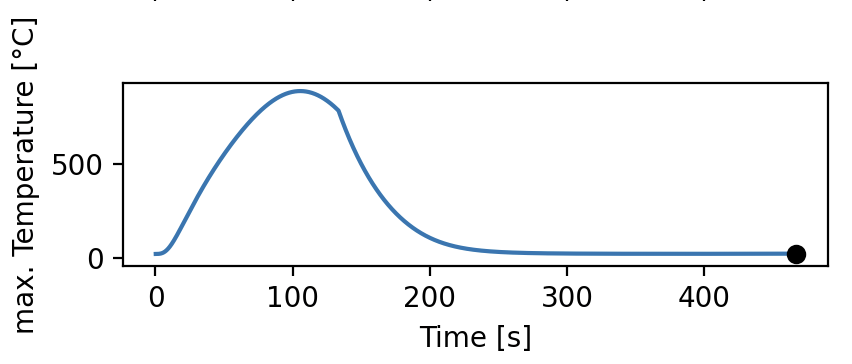
\includegraphics[width=.8\textwidth]{images/max_temp.png}
        \caption{Maximale Temperatur der Raketenspitze über der Zeit}
        \label{fig:max_temp}
    \end{figure}

    \item \textbf{Berechnen Sie die optimale Stufung für diese Raketenkonfiguration (gleiche Startmasse, gleicher Strukturindex). Wie hoch ist die potentielle Steigerung der Nutzlast?}\\
    
    Wie in der Vorlesung gezeigt, ist eine optimale Stufung bei gleichem spezifischem Impuls aller Stufen dann gegeben, wenn das Masseverhältnis der Start- zu Endmassen aller Stufen gleich ist. Folgende Gleichung beschreibt die Masse der Nutzlast $m_{p}$ in Abhängigkeit von der Startmasse $M_0$, der Austrittsgeschwindigkeit $u_e$, so wie dem benötigten $\Delta v$ und dem Strukturindex $N_s$ unter dieser Vorraussetzung:
    \begin{equation}
        \frac{m_p}{M_0} = \left[ \frac{(1-\epsilon) \exp{\left( \frac{\Delta v}{u_e N_s}\right) }}{1-\epsilon \exp{ \left(\frac{\Delta v}{u_e N_s}\right)}} \right]^{-N_s}.
    \end{equation}
    $\epsilon$ ist der Strukturindex, also das Verhältnis von Strukturmasse zur Summe von Struktur und Treibstofmasse einer Stufe. Die Nutzlast kann bei einer festen Startmasse von 285 t, einem Strukturindex von $\frac{1}{11}$ und einem $\Delta v$ von 9366 m/s auf 10.142 t erhöht werden. \\

    Wenn statt dem $\Delta v$ ein Zielorbit vorgegeben ist, kann nicht mehr einfach die Nutzlast berechnet werden, da die benötigte Geschwindigkeitsänderung von der Rakete abhängt. Für diesen Fall wird eine Abschätzung der Nutzlast über den nicht verwendeten Treibstoff gemacht.

    Die optimale Stufung für die Konfiguration mit einer 10 t schweren Nutzlast ist in der folgenden Tabelle dargestellt:
    \begin{center}
        \begin{tabular}{c | c | c | c | c}
            Stufe & Strukturmasse [t] & Treibstoffmasse [t] & $\epsilon$ & Payload [t] \\
            \midrule
            1 & 21.05 & 210.5 & 3.83 &  \\
            2 & 3.95 & 39.5 & 3.83 & 10 \\
        \end{tabular}
    \end{center}
    Diese wurde numerisch ermittelt, der Code dafür befindet sich in \textit{stage.py}. Nun muss für die neue Raketenkonfiguration ein neues Flugprofil gefunden werden. Dafür wurde die Simulation so angepasst, dass es möglich ist den Antrieb auszuschalten und für ein Zirkularisierungsmanöver erneut anzuschalten. So kann effizienter ein nahezu kreisförmiger Orbit gefunden werden. Mit einer TVC von $8.4 ^\circ$ zwischen 1 km und 9.25 km konnte ein Orbit mit einer Apoapsis von ca. 272.2 km und einer Periapsis von 268.5 km erreicht werden, indem ein Zirkularisierungsmanöver durchgeführt wird. Es sind dann 773 kg Treibstoff übrig, was eine große Verbesserung gegenüber den aus Aufgabe 1 ermittelten Wert darstellt. Mit diesem Wert könnte man nun mit dem gleichen Prozess iterativ die optimale Stufung annähern, im Rahmen dieses Praktikums soll aber nur eine Iteration durchgeführt werden.
    


\end{enumerate}

\appendix
\section{Code}
Der Code für den Raketen-Flugsimulator ist auf GitHub verfügbar und im Anhang der Email zur Abgage zu finden. Der Link zum Repository ist:

\url{https://github.com/LoloSpirit/rocket_flight_sim/tree/main}.


\end{document}